\documentclass[10pt]{article}
\usepackage{fullpage}
\usepackage{array}
\usepackage{amsmath,amssymb,amsfonts,mathrsfs,amsthm}
\usepackage[utf8]{inputenc}
\usepackage{listings}
\usepackage{mathtools}
\usepackage{pdfpages}
\usepackage[textsize=footnotesize,color=green]{todonotes}
\usepackage{bm}
\usepackage{tikz}
\usepackage[normalem]{ulem}

\usepackage{graphicx}
\usepackage{subfigure}

\usepackage{color}
\usepackage{pdflscape}
\usepackage{pifont}

\usepackage{bibentry}
\nobibliography*

\renewcommand{\topfraction}{0.85}
\renewcommand{\textfraction}{0.1}
\renewcommand{\floatpagefraction}{0.75}

\newcommand{\vect}[1]{\ensuremath\boldsymbol{#1}}
\newcommand{\tensor}[1]{\underline{\vect{#1}}}
\newcommand{\del}{\triangle}
\newcommand{\grad}{\nabla}
\newcommand{\curl}{\grad \times}
\renewcommand{\div}{\grad \cdot}
\newcommand{\ip}[1]{\left\langle #1 \right\rangle}
\newcommand{\eip}[1]{a\left( #1 \right)}
\newcommand{\pd}[2]{\frac{\partial#1}{\partial#2}}
\newcommand{\pdd}[2]{\frac{\partial^2#1}{\partial#2^2}}

\newcommand{\circone}{\ding{192}}
\newcommand{\circtwo}{\ding{193}}
\newcommand{\circthree}{\ding{194}}
\newcommand{\circfour}{\ding{195}}
\newcommand{\circfive}{\ding{196}}

\newcommand{\Reyn}{\rm Re}

\newcommand{\bs}[1]{\boldsymbol{#1}}
\DeclareMathOperator{\diag}{diag}

\newcommand{\equaldef}{\stackrel{\mathrm{def}}{=}}

\newcommand{\tablab}[1]{\label{tab:#1}}
\newcommand{\tabref}[1]{Table~\ref{tab:#1}}

\newcommand{\theolab}[1]{\label{theo:#1}}
\newcommand{\theoref}[1]{\ref{theo:#1}}
\newcommand{\eqnlab}[1]{\label{eq:#1}}
\newcommand{\eqnref}[1]{\eqref{eq:#1}}
\newcommand{\seclab}[1]{\label{sec:#1}}
\newcommand{\secref}[1]{\ref{sec:#1}}
\newcommand{\lemlab}[1]{\label{lem:#1}}
\newcommand{\lemref}[1]{\ref{lem:#1}}

\newcommand{\mb}[1]{\mathbf{#1}}
\newcommand{\mbb}[1]{\mathbb{#1}}
\newcommand{\mc}[1]{\mathcal{#1}}
\newcommand{\nor}[1]{\left\| #1 \right\|}
\newcommand{\snor}[1]{\left| #1 \right|}
\newcommand{\LRp}[1]{\left( #1 \right)}
\newcommand{\LRs}[1]{\left[ #1 \right]}
\newcommand{\LRa}[1]{\left\langle #1 \right\rangle}
\newcommand{\LRb}[1]{\left| #1 \right|}
\newcommand{\LRc}[1]{\left\{ #1 \right\}}

\newcommand{\Grad} {\ensuremath{\nabla}}
\newcommand{\Div} {\ensuremath{\nabla\cdot}}
\newcommand{\Nel} {\ensuremath{{N^\text{el}}}}
\newcommand{\jump}[1] {\ensuremath{\LRs{\![#1]\!}}}
\newcommand{\uh}{\widehat{u}}
\newcommand{\fnh}{\widehat{f}_n}
\renewcommand{\L}{L^2\LRp{\Omega}}
\newcommand{\pO}{\partial\Omega}
\newcommand{\Gh}{\Gamma_h}
\newcommand{\Gm}{\Gamma_{-}}
\newcommand{\Gp}{\Gamma_{+}}
\newcommand{\Go}{\Gamma_0}
\newcommand{\Oh}{\Omega_h}

\newcommand{\eval}[2][\right]{\relax
  \ifx#1\right\relax \left.\fi#2#1\rvert}

\def\etal{{\it et al.~}}


\def\arr#1#2#3#4{\left[
\begin{array}{cc}
#1 & #2\\
#3 & #4\\
\end{array}
\right]}
\def\vecttwo#1#2{\left[
\begin{array}{c}
#1\\
#2\\
\end{array}
\right]}
\def\vectthree#1#2#3{\left[
\begin{array}{c}
#1\\
#2\\
#3\\
\end{array}
\right]}
\def\vectfour#1#2#3#4{\left[
\begin{array}{c}
#1\\
#2\\
#3\\
#4\\
\end{array}
\right]}

\newcommand{\G} {\Gamma}
\newcommand{\Gin} {\Gamma_{in}}
\newcommand{\Gout} {\Gamma_{out}}


\title{Ideas}
\author{Jesse Chan}
\begin{document}

\section{Weak boundary conditions}

We can derive weak boundary conditions for the convection-diffusion equation.  The motivation is that, as $\epsilon \rightarrow 0$, the problem should converge to the pure convection problem, which has boundary conditions $\left.u\right|_{\Gamma_{\rm in}} = u_{\rm in}$ and $\left.e\right|_{\Gamma_{\rm out}} = 0$.  We would like our variational formulation for convection-diffusion problem to converge to these spaces as $\epsilon \rightarrow 0$.  

For standard convection-diffusion, we have
\[
b(u,v) = \LRp{-u,\beta\cdot\grad v}_{\L} + \epsilon\LRp{\grad u,\grad v}_{\L} - \epsilon\LRa{\pd{u}{n},v}_{\Gamma_{\rm in}}.
\]
Imposition of weak boundary conditions is similar to Nitsche's method for weak boundary condition imposition, though it is lacking the penalty term and mesh-dependent parameters found in his method.  
\[
b(u,v) = \LRp{-u,\beta\cdot\grad v}_{\L} + \epsilon\LRp{\grad u,\grad v}_{\L} - \epsilon\LRa{\pd{u}{n},v}_{\Gamma_{\rm in}} - \epsilon\LRa{u,\pd{v}{n}}_{\Gamma_{\rm out}}.
\]
The term $\epsilon\LRa{u,\pd{v}{n}}_{\Gamma_{\rm out}}$ weakly enforces the outflow condition on $u$, similarly to the way in which the term $\epsilon\LRa{\pd{u}{n},v}_{\Gamma_{\rm in}}$ enforces a weak boundary condition on the test space.  

\begin{figure}
\centering
\subfigure[$\epsilon = .1$]{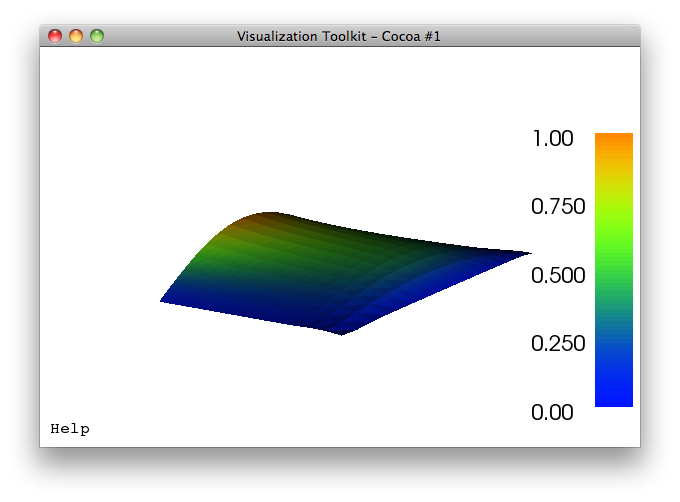
\includegraphics[width=8cm]{figs/weakBCs/eps1e1}}
\subfigure[$\epsilon = .01$]{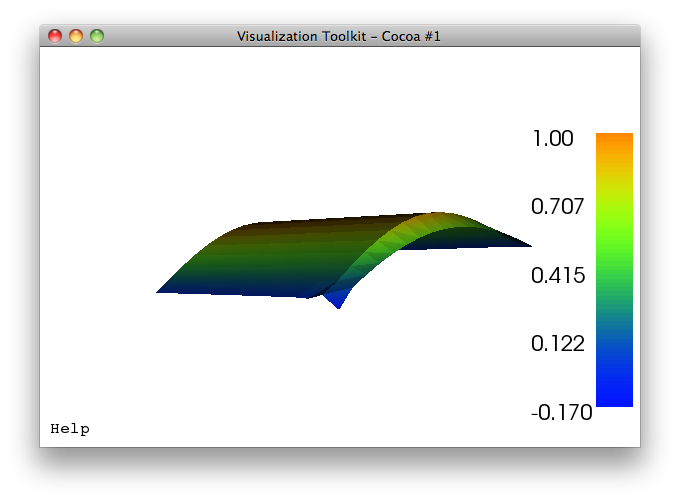
\includegraphics[width=8cm]{figs/weakBCs/eps1e2}}
\subfigure[$\epsilon = .001$]{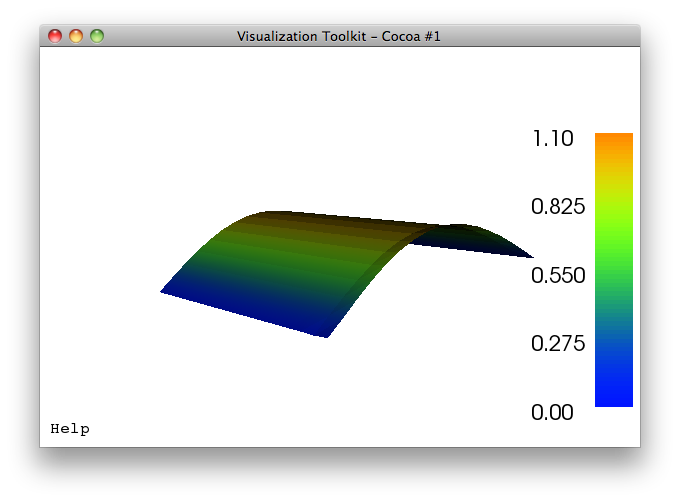
\includegraphics[width=8cm]{figs/weakBCs/eps1e3}}
\subfigure[$\epsilon = .0001$]{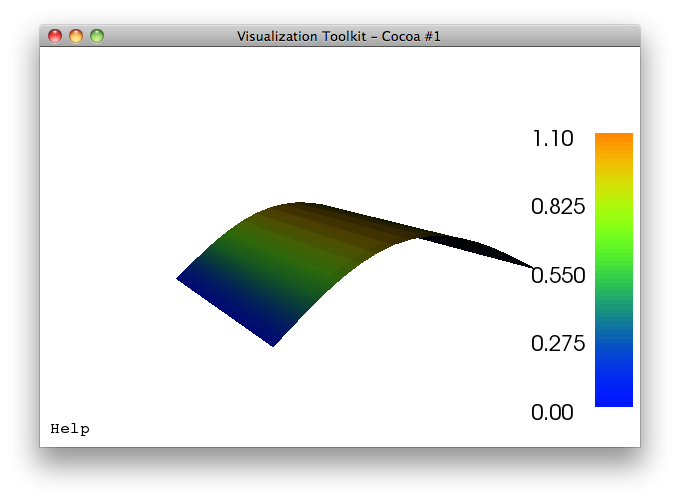
\includegraphics[width=8cm]{figs/weakBCs/eps1e4}}

\end{figure}

\section{Deriving the trial norm}

Strong convection-diffusion: 
\[
\div{\beta u} + \epsilon\del u = f
\]
Weak form: $v\in H^1_{\rm out}$
\[
b(u,v) = \LRp{-u,\beta\cdot\grad v}_{\L} + \epsilon\LRp{\grad u,\grad v}_{\L} - \epsilon\LRa{\pd{u}{n},v}_{\Gamma_{\rm in}}
\]
Test norm:
\[
\nor{v}^2_V = \nor{\beta\cdot\grad v}_{\L}^2 + \epsilon\nor{\grad{v}}^2_{\L} + \epsilon\nor{v}^2_{\Gamma_{\rm in}}
\]
Cauchy-Schwarz gives 
\[
\LRb{b(u,v)} \leq \nor{u} \nor{\beta\cdot\grad v} + \epsilon\nor{\grad{u}}\nor{\grad v} + \epsilon\nor{\pd{u}{n}}_{\Gamma_{\rm in}}\nor{v}_{\Gamma_{\rm in}}.
\]
Equality holds if each of the paired normed terms are equal.  This may not be possible given the trace terms --- the supremum of the trace term may not be representable using our trace spaces.  

Discrete Cauchy-Schwarz gives
\[
\LRb{b(u,v)} \leq \LRp{\nor{u}^2+\epsilon\nor{\grad{u}}^2 + \epsilon\nor{\pd{u}{n}}_{\Gamma_{\rm in}}}^{1/2}\LRp{\nor{\beta\cdot\grad v}^2+\epsilon\nor{\grad{v}}^2 + \epsilon\nor{v}_{\Gamma_{\rm in}}}^{1/2}
\]
Equality here is easier to show.  

If equality of the first Cauchy-Schwarz inequality holds, would it be correct then to claim
\[
\sup_{v\in H^1_{\rm out}\setminus\LRc{0}} \frac{ b(u,v)}{\nor{v}_V} =  \LRp{\nor{u}^2+\epsilon\nor{\grad{u}}^2 + \epsilon\nor{\pd{u}{n}}_{\Gamma_{\rm in}}}^{1/2}?
\]

\end{document}
